\documentclass{sciposter}


\usepackage{epsfig}
\usepackage{amsmath}
\usepackage{amssymb}
\usepackage{multicol}
%\usepackage{fancybullets}

\newtheorem{Def}{Definition}

%\definecolor{BoxCol}{rgb}{0.9,0.9,0.9}
% uncomment for grey background to \section boxes 
% for use with default option boxedsections

%\definecolor{BoxCol}{rgb}{0.9,0.9,1}
% uncomment for light blue background to \section boxes 
% for use with default option boxedsections

%\definecolor{SectionCol}{rgb}{0,0,0.5}
% uncomment for dark blue \section text 






\title{Reminder}

% Note: only give author names, not institute
\author{Lei Ma}
 
% insert correct institute name
\institute{Department of Physics and Astronomy,\\
           University of New Mexico\\}

\email{leima@unm.edu}  % shows author email address below institute

%\date is unused by the current \maketitle


% The following commands can be used to alter the default logo settings
%\leftlogo[0.9]{logoWenI}{  % defines logo to left of title (with scale factor)
%\rightlogo[0.52]{RuGlogo}  % same but on right

% NOTE: This will require presence of files logoWenI.eps and RuGlogo.eps, 
% or other supported format in the current directory  
%%%%%%%%%%%%%%%%%%%%%%%%%%%%%%%%%%%%%%%%%%%%%%%%%%%%%%%%%%%%%%%%%%%%%%%%%%%%%%%%
%%% Begin of Document



\begin{document}
%define conference poster is presented at (appears as footer)

\conference{{\bf 2015-11-10}}

%\LEFTSIDEfootlogo  
% Uncomment to put footer logo on left side, and 
% conference name on right side of footer

% Some examples of caption control (remove % to check result)

%\renewcommand{\algorithmname}{Algoritme} % for Dutch

%\renewcommand{\mastercapstartstyle}[1]{\textit{\textbf{#1}}}
%\renewcommand{\algcapstartstyle}[1]{\textsc{\textbf{#1}}}
%\renewcommand{\algcapbodystyle}{\bfseries}
%\renewcommand{\thealgorithm}{\Roman{algorithm}}

%\maketitle

%%% Begin of Multicols-Enviroment
\begin{multicols}{3}

%%% General

\section{General}


\subsection{Units and Conventions}

\begin{enumerate}
\item Energy and temperature: \begin{equation}
\frac{1}{40}\mathrm{eV} = 300\mathrm{K} k_B .
\end{equation}
\item Natural units: energy is related to length by
\begin{equation}
1\mathrm{fm}\times 197\mathrm{MeV}=\hbar c = 1.
\end{equation}
\item For light, energy 1eV corresponds to wavelength $1.24\mathrm{\mu m}$.
\item Pauli matrices are
\begin{equation}
    \sigma_1 = \begin{pmatrix} 0 & 1 \\ 1 & 0 \end{pmatrix}, \sigma_2 = \begin{pmatrix} 0 & -i \\ i & 0 \end{pmatrix},\sigma_3 = \begin{pmatrix} 1 & 0 \\ 0 & -1 \end{pmatrix}.
\end{equation}
\end{enumerate}




\subsection{Check Results}

\begin{enumerate}
    \item Are the dimensions correct?
    \item Does the limits of the result make sense?
    \item Does the result make sense when the complexity of the system is removed?
    \item Is it the right basis to draw a conclusion?
\end{enumerate}




%%% Field Theory


\section{Field Theory}


\subsection{Equations of Motion}

\begin{itemize}
\item Dirac Equation
\begin{equation}
i\hbar \gamma^\mu \partial_\mu \psi - m c \psi = 0
\end{equation}
\item Klein Gordon Equation
\begin{equation}
\frac {1}{c^2} \frac{\partial^2}{\partial t^2} \psi - \nabla^2 \psi + \frac {m^2 c^2}{\hbar^2} \psi = 0
\end{equation}
\end{itemize}





%%% Neutrinos

\section{Neutrinos}


\subsection{Fundamental Parameters}

\begin{itemize}
\item Mixing angles
\begin{align}
\sin^2 2\theta_{12} & = 0.857 \pm 0.024 \\
\sin^2 2\theta_{23} & > 0.95 \\
\sin^2 2\theta_{13} & = 0.095 \pm 0.010 \\
\end{align}
\item Masses
\begin{align}
\Delta m_{12}^2 &= \Delta m_{sol}^2 = 7.53_{-0.18}^{+0.18} \times 10^{-5} \mathrm{eV}^2 \\
\lvert\Delta m_{31}^2\rvert & = \Delta m_{atm}^2 = 2.44_{-0.06}^{+0.06}\times 10^{-3} \mathrm{eV^2}
\end{align}

\end{itemize}

\subsection{Nuclear Reactions}


\begin{figure}[h]
\centering
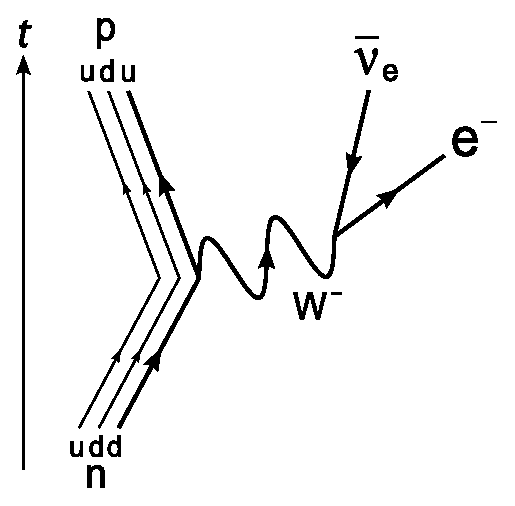
\includegraphics[width=\columnwidth]{assets/Beta_Negative_Decay.eps}
\caption{Feynman diagram of beta decay. The charged current weak interaction boson in this case is a $W^-$. Credit: Joel Holdsworth, within public domain.}
\label{fig:Beta_Negative_Decay}
\end{figure}
i

\begin{table}[ht]
\centering
 \begin{tabular}{|c | c | c|} 
 \hline
 Reaction & Equation & Boson   \\ [0.5ex] 
 \hline
 Electron emission & ${}^A_Z X \to {}^A_{Z+1}X + e^- +\bar \nu_e$ & $W$  \\ 
 Positron emission & ${}^A_Z X \to {}^A_{Z-1}X + e^+ + \nu_e$ & $W$  \\
 Electron capture & ${}^A_Z X + e^- \to {}^A_{Z-1}X  + \nu_e$ &  $W$ \\
 Positron capture & ${}^A_Z X + e^+ \to {}^A_{Z+1}X  + \bar\nu_e$ &  $W$ \\
 [0.5ex] 
 \hline

 Electron annihilation &  $e^- + e^+  \to \nu_e + \bar\nu_e $  & $W$ \\
 Electron annihilation &  $e^- + e^+  \to \nu + \bar\nu $  & $Z$ \\
 [0.5ex] 
 \hline

  Neutrino capture & ${}^A_{Z}X + \overset{(-)}{\nu_e} \to {}^A_{Z\mp 1}X + e^\pm $ & W\\
  [1ex] 
 \hline
 $e^-\nu$ scattering & $e^- + \overset{(-)}{\nu_e} \to e^- + \overset{(-)}{\nu_e} $ &  $W$ \\
 $e^-\nu$ scattering & $e^{\pm} + \overset{(-)}{\nu_e} \to e^{\pm} + \overset{(-)}{\nu_e} $ &  $Z$ \\
 Neutrino scattering & $ {}^A_Z X + \overset{(-)}{\nu} \to {}^A_Z X + \overset{(-)}{\nu} $ &  Z\\
 [0.5ex] 
 \hline
 
 Bremsstrahlung & $N+N\rightleftharpoons N+N + \nu + \bar\nu$ & \\
 Annihilation & $e^+e^- \rightleftharpoons \nu + \bar \nu$   & \\
 Neutrino annihilation & $\nu + \bar \nu  \rightleftharpoons \nu + \bar \nu $   &  \\
 [0.5ex] 
 \hline
 \end{tabular}
 \caption{Neutrino related nuclear or leptonic reactions}
\label{table:Neutrino_Reactions}
\end{table}



\subsection{Neutrino Mixing}

\begin{figure}
\centering
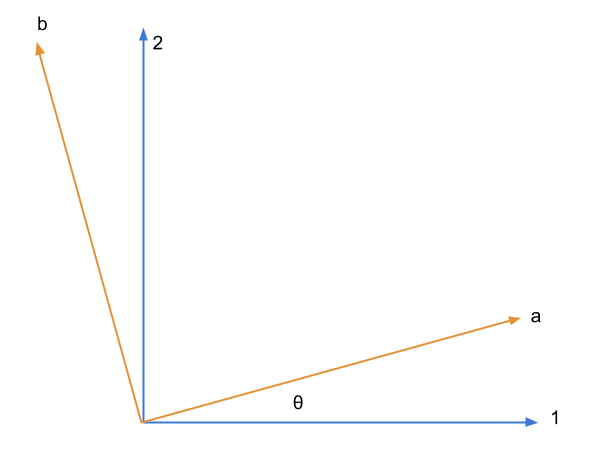
\includegraphics[width=\columnwidth]{assets/neutrinoMixingAngle.png}
\caption{Neutrino mixing. Blue states ($\{1,2\}$) are the VACUUM energy eigenstates while the orange states ($\{a,b\}$) are the flavor eigenstates. Blue: electron flavor; Red: the other flavor.}
\label{fig:neutrinoMixingAngle}
\end{figure}




%%% Numerical

\section{Numerical}

\subsection{Check You Code}
Check the code step by step:

\begin{itemize}
\item Vacuum oscillation amplitude and frequency
\item Constant matter potential oscillation amplitude and frequency
\item MSW resonance
\end{itemize}


\subsection{Zen of Python}

\verb+import this+

\begin{enumerate}
\item     Beautiful is better than ugly.
\item     Explicit is better than implicit.
\item     Simple is better than complex.
\item     Complex is better than complicated.
\item     Flat is better than nested.
\item     Sparse is better than dense.
\item     Readability counts.
\item     Special cases aren't special enough to break the rules.
\item     Although practicality beats purity.
\item     Errors should never pass silently.
\item     Unless explicitly silenced.
\item     In the face of ambiguity, refuse the temptation to guess.
\item     There should be one-- and preferably only one --obvious way to do it.
\item     Although that way may not be obvious at first unless you're Dutch.
\item     Now is better than never.
\item     Although never is often better than *right* now.
\item     If the implementation is hard to explain, it's a bad idea.
\item     If the implementation is easy to explain, it may be a good idea.
\item     Namespaces are one honking great idea -- let's do more of those!
\end{enumerate}



\end{multicols}

\end{document}

